\documentclass{beamer}

\beamertemplatenavigationsymbolsempty

\usepackage[utf8]{inputenc}
\usepackage{listings}
\usepackage{minted}
\usepackage{tikz}

\usetikzlibrary{graphs,quotes,arrows.meta}
\definecolor{themegreen}{RGB}{0,100,0}
\definecolor{themelightgreen}{RGB}{230,239,230}
\definecolor{themelightblue}{RGB}{215,215,240}

% set graphics path to figure
\graphicspath{{./figures/}}

\usetheme{Madrid}
\usecolortheme{seahorse}
%Information to be included in the title page:
\title[DataFlowTasks] % optional short title
{DataFlowTasks.jl}

% Custom commands
\newcommand{\DFT}{\texttt{DataFlowTasks.jl}}

\subtitle{Julia \texttt{Task}s which automatically handle data-dependencies}

\author[Faria, Févotte] % short version of authors
{Luiz~M.~Faria\inst{1} \and François Févotte\inst{2}}

\institute[]
{
    \inst{1}%
    Chargé de recherche INRIA\\
    POEMS Laboratory
    \and
    \inst{2}%
    Chief Scientist\\
    TriScale innov
}

\AtBeginSection[]
{
    \begin{frame}
        \frametitle{Table of Contents}
        \tableofcontents[currentsection]
    \end{frame}
}

\date{\today}

\titlegraphic{
  
\includegraphics[height=0.5cm]{inr_logo_rouge.png}\hspace{2em}
  
\includegraphics[height=0.5cm]{poems_logo.png}\hspace{2em}
  
\includegraphics[height=0.5cm]{triscale_couleur_texteadroite.png}
}

\begin{document}

\frame{\titlepage}

% small textsize on frame
\begin{frame}[fragile]
\frametitle{Overview}

\begin{itemize}
    \item \DFT{} is a Julia package dedicated to parallel programming on multi-core shared memory CPUs.
    \item Automatically infer \texttt{Task} interdependencies based on user annotations (\mintinline{julia}{@R, @W, @RW}).
    \item Heavily inspired by task programming libraries such as StarPU.
    \item Simple API: \mintinline{julia}{@dspawn} macro.
\end{itemize}
%
\begin{columns}[t]
\column{0.3\textwidth}
\begin{exampleblock}{}
\begin{minted}[fontsize=\footnotesize]{julia}
function foo!(A)
  fill!(A, 0)          
  view(A, 1:2) .+= 2   
  view(A, 3:4) .+= 3   
  sum(A)               
end
\end{minted}
\end{exampleblock}
\center 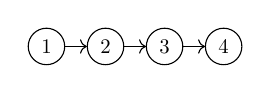
\begin{tikzpicture}[scale=0.75, every node/.style={transform shape}]
\graph[nodes={draw,circle}] {
1 -> 2 -> 3 -> 4
};
\end{tikzpicture}
 
\column{0.6\textwidth}

\begin{exampleblock}{}
\begin{minted}[fontsize=\footnotesize]{julia}
function foo!(A)
  @dspawn fill!(@W(A), 0)         # task 1
  @dspawn @RW(view(A, 1:2)) .+= 2 # task 2
  @dspawn @RW(view(A, 3:4)) .+= 3 # task 3
  @dspawn sum(@R(A))              # task 4
end
\end{minted}
\end{exampleblock}
\center 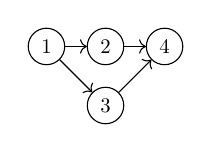
\begin{tikzpicture}[scale=0.75, every node/.style={transform shape}]
\graph[nodes={draw,circle}] {
  1 -> {2, 3} -> 4
};
\end{tikzpicture}

\end{columns}

% In this presentation, we will explore the features and benefits of \DFT{} in the context of efficient parallel programming.

\end{frame}

\begin{frame}
    \frametitle{Table of Contents}
    \tableofcontents
\end{frame}

\section{Introduction and high-level usage}

\subsection{Task based parallelism in Julia}

\begin{frame}[fragile]
\frametitle{Task based parallelism}
\begin{itemize}
    \item A task is a unit of execution or a unit of work
    \item \mintinline{julia}{Task} objects can be created using \mintinline{julia}{@task}
    \item Once created, \mintinline{julia}{Task} objects must be scheduled for execution
    \item Usually, \mintinline{julia}{Task}s are created + scheduled using \mintinline
    {julia}{@spawn}
    \item \alert{Responsibility of synchronizing tasks is left to the programmer}
\end{itemize}

\begin{columns}
\column{0.8\textwidth}    

\begin{example}[%
  \only<1>{Sequential}%
  \only<2>{Synchronizing tasks with return values}%
  \only<3>{Synchronizing tasks with explicit barriers}%
  ]
\begin{onlyenv}<1>
\begin{minted}[beameroverlays]{julia}
              # Task
A = zeros(4)     # 1 - Initialization
A[1:2] .+= 2     # 2 - Work on first half
A[3:4] .+= 3     # 3 - Work on second half
res = sum(A)     # 4 - Reduction
                 #
\end{minted}
\end{onlyenv}
\begin{onlyenv}<2>
\begin{minted}[beameroverlays]{julia}
                                         # Task
t1 = @spawn zeros(4)                        # 1
t2 = @spawn (A = fetch(t1); A[1:2] .+ 2)    # 2
t3 = @spawn (A = fetch(t1); A[3:4] .+ 3)    # 3
t4 = @spawn sum(fetch(t2)) + sum(fetch(t3)) # 4
fetch(t4) # get result
\end{minted}
\end{onlyenv}
\begin{onlyenv}<3>
\begin{minted}[beameroverlays]{julia}    
A = rand(4)                              # Task
t1 = @spawn fill!(A,0)                      # 1
t2 = @spawn (wait(t1); view(A,1:2) += 2)    # 2
t3 = @spawn (wait(t1); view(A,3:4) += 3)    # 3
t4 = @spawn (wait(t2); wait(t3); sum(A))    # 4
fetch(t4) # get result
\end{minted}
\end{onlyenv}
\end{example}

\column{0.15\textwidth}

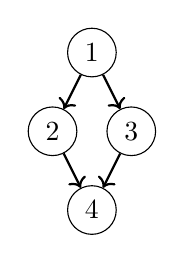
\begin{tikzpicture}
    % Nodes
    \node[circle, draw] (1) at (0, 0) {1};
    \node[circle, draw] (2) at (-0.5, -1) {2};
    \node[circle, draw] (3) at (0.5, -1) {3};
    \node[circle, draw] (4) at (0, -2) {4};
    % Edges
    \draw[->, thick] (1) -- (2);
    \draw[->, thick] (1) -- (3);
    \draw[->, thick] (2) -- (4);
    \draw[->, thick] (3) -- (4);
\end{tikzpicture}

\end{columns}

\end{frame}

\subsection{Motivation}

\begin{frame}[fragile]
\frametitle{Motivation}

\begin{itemize}
    \item Reasoning about \mintinline{julia}{Task} interdependencies can be
    challenging
    \item Specially for algorithms making constant re-use of data   
    \item Sometimes, it is simpler to reason about how \mintinline{julia}{Task}s depend on data than how \mintinline{julia}{Task}s depend on each other
\end{itemize}

\begin{example}[Synchronizing tasks]
\begin{minted}[fontsize=\small]{julia}    
A = rand(4)
t1 = @spawn fill!(A,0)                   # RW access to A
t2 = @spawn (wait(t1); view(A,1:2) += 2) # RW access to A[1:2]   
t3 = @spawn (wait(t1); view(A,3:4) += 3) # RW access to A[3:4]
t4 = @spawn (wait(t2); wait(t3); sum(A)) # R access to A
fetch(t4)
\end{minted}
\end{example}

\begin{itemize}
  \item<2-> \alert{Would like to declare only the task-to-data dependencies}
\end{itemize}

\end{frame}

\subsection{Basic idea}

\begin{frame}[fragile]

\frametitle{Basic idea}
\begin{enumerate}
    \item \textcolor<4->{lightgray}{Extract data dependency from user annotations}
    \item \textcolor<1-3,10->{lightgray}{Infer task dependency from data dependency}
    \item \textcolor<1-9>{lightgray}{Schedule tasks with inferred dependencies}
\end{enumerate}

\center
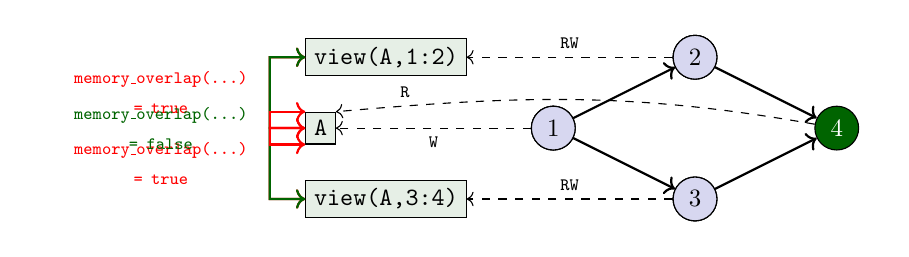
\begin{tikzpicture}[scale=0.9, every node/.style={transform shape}]
  % Tasks
  \node<2->[circle, draw] (1) at (0,  0) {1};
  \node<2>[circle, draw, fill=themegreen, text=white] at (0,  0) {1};
  \node<4,6,9>[circle, draw, fill=themelightblue] at (0,  0) {1};
  
  \node<3->[circle, draw] (2) at (2,  1) {2};
  \node<3-4>[circle, draw, fill=themegreen, text=white] at (2,  1) {2};
  \node<5,8>[circle, draw, fill=themelightblue] at (2,  1) {2};
  
  \node<5->[circle, draw] (3) at (2, -1) {3};
  \node<5-6>[circle, draw, fill=themegreen, text=white] at (2, -1) {3};
  \node<7>[circle, draw, fill=themelightblue] at (2, -1) {3};

  \node<7->[circle, draw, fill=themegreen, text=white] (4) at (4,  0) {4};
  
  % Data
  \node<1->[rectangle, draw, fill=themelightgreen, anchor=west] (A)  at (-3.5,  0) {\texttt{A}};
  \node<3->[rectangle, draw, fill=themelightgreen, anchor=west] (A1) at (-3.5,  1) {\texttt{view(A,1:2)}};
  \node<5->[rectangle, draw, fill=themelightgreen, anchor=west] (A2) at (-3.5, -1) {\texttt{view(A,3:4)}};
  
  % Task -> Data dependencies
  \draw<2->[->, dashed] (1) -- node[midway, below]{\scriptsize\ttfamily W} (A);
  \draw<3->[->, dashed] (2) -- node[midway, above]{\scriptsize\ttfamily RW} (A1) ;
  \draw<5->[->, dashed] (3) -- node[midway, above]{\scriptsize\ttfamily RW} (A2);
  \draw<7-> (4) edge[out=170, in=5, dashed, ->] node[pos=0.87, above]{\scriptsize\ttfamily R} (A.north east);
  
  % Task -> Task dependencies
  \draw<4->[->, thick] (1) -- (2);
  \draw<6->[->, thick] (1) -- (3);
  \draw<8->[->, thick] (2) -- (4);
  \draw<7->[->, thick] (3) -- (4);
  
  % Data <-> Data dependencies
  \draw<1-> (A.west)  ++(-0.5,0) node (Aw)  {};
  \draw<3-> (A1.west) ++(-0.5,0) node (A1w) {};
  \draw<5-> (A2.west) ++(-0.5,0) node (A2w) {};
  \draw<4,8>[<->, thick, red] (A.west)  -- (Aw.center)
  -- node[midway,left,text width=8em,align=center]{\scriptsize\ttfamily memory\_overlap(...) = true} (A1w.center) -- (A1.west);
  \draw<6,7>[<->, thick, red] (A.west)  -- (Aw.center)
  -- node[midway,left,text width=8em,align=center]{\scriptsize\ttfamily memory\_overlap(...) = true} (A2w.center) -- (A2.west);
  \draw<5>[<->, thick, themegreen] (A1.west) -- (A1w.center)
  -- node[midway,left,text width=8em,align=center]{\scriptsize\ttfamily memory\_overlap(...) = false} (A2w.center) -- (A2.west);
  \draw<9>[<->, thick, red] (A.south west) -- ++(-0.5,0) |- (A.north west);

  % Bounding box
  \node at (-7.3,-1.3) {};
  \node at (4.5,1.3) {};
\end{tikzpicture}

\begin{columns}[T]
  \column{0.42\textwidth}
\begin{exampleblock}{User-written code}
\begin{minted}[fontsize=\footnotesize,escapeinside=||,beameroverlays=true]{julia}
|\onslide<1->|A = rand(4)
|\onslide<2->|@dspawn fill!(@W(A),0)
|\onslide<3->|@dspawn @RW(view(A,1:2)) += 2
|\onslide<5->|@dspawn @RW(view(A,3:4)) += 3
|\onslide<7->|t4 = @dspawn sum(@R(A))
|\onslide<7->|fetch(t4)|\onslide<1->|
\end{minted}    
\end{exampleblock}
  
  \column{0.50\textwidth}
\begin{onlyenv}<4-9>
  \begin{exampleblock}{Behind the scenes: DAG}
\begin{minted}[fontsize=\footnotesize,escapeinside=||]{julia}
# Note the quadratic complexity!
for i in 1:N, j in i:-1:1
  # Detect conflict between i and j
  for di in data(i), dj in data(j)
    if memory_overlap(di, dj)
      add_edge(j, i)
\end{minted}
\end{exampleblock}
\end{onlyenv}
\begin{onlyenv}<10>
\begin{exampleblock}{Behind the scenes: task scheduling}
\begin{minted}[fontsize=\footnotesize]{julia}
t4 = Threads.@spawn begin
  wait(t2); wait(t3)
  sum(A)
end
\end{minted}
\end{exampleblock}
\end{onlyenv}
\end{columns}

% \alert{Note the quadratic complexity in the number of tasks!}

\end{frame}

\subsection{Simple example: parallel merge sort}

\begin{frame}
\frametitle{Simple example}
\center \href{run:./sort.slides.html}{\LARGE{Demo: parallel merge sort}}

\end{frame}

\section{\mintinline{julia}{Implementation details}}

\begin{frame}{Main types}

The package revolves around three main types:
\begin{itemize}
  \item <1->\mintinline{julia}{DataFlowTask}: wrapper around a
  \mintinline{julia}{Task} with user-declared data dependencies
  \item <2->\mintinline{julia}{DAG}: graph data
  structure to represent dependencies between \mintinline{julia}{DataFlowTask}s
  \item <3->\mintinline{julia}{TaskGraph}: a
  \mintinline{julia}{DAG} and some helper functions/workers to manage it

\end{itemize}

\begin{alertblock}<4->{}
  Next: some technical details about their
  implementation.
\end{alertblock}

\end{frame}

\subsection{\mintinline{julia}{DataFlowTask}}

\begin{frame}[fragile]

\frametitle{\texttt{DataFlowTask}: \mintinline{julia}{@dspawn} macro}

\texttt{DataFlowTask}s are created using \mintinline{julia}{@dspawn}. The macro
does the following:

\begin{itemize}
    \item <2->Scan the \mintinline{julia}{Expr} for \mintinline{julia}{@R, @W, @RW} annotations
    \item <3->Create a \mintinline{julia}{data} and \mintinline{julia}{access_mode}
    tuple
    \item <4->Remove annotations from the \mintinline{julia}{Expr}
    \item <5->Parse keyword arguments    
    \item <6->Create an anonymous function wrapping the new \mintinline{julia}{Expr}
    \item <7->Insert a call to \mintinline{julia}{DataFlowTask} constructor
\end{itemize}

\begin{columns}[T]

\column{0.45\textwidth}    
\begin{exampleblock}{User-written code}    
\begin{minted}{julia}
@dspawn(foo!(@W(B), @R(A)),
        label="foo!")
\end{minted}
\end{exampleblock}

\column{0.4\textwidth}    

\begin{exampleblock}<8->{Macro expansion (approx.)}    
\begin{minted}{julia}
_t = DataFlowTask(
       () -> foo!(B, A),
       (B, A),
       (WRITE, READ);
       label="foo!")
spawn(_t)
\end{minted}
\end{exampleblock}

\end{columns}
%

\end{frame} 

\begin{frame}[fragile]

\frametitle{\texttt{DataFlowTask} structure}

\small{\alert{Inner-constructor of \mintinline{julia}{DataFlowTask} handles much of
the insertion/removal logic:}}

\hrulefill
\begin{minted}[fontsize=\footnotesize]{julia}
mutable struct DataFlowTask
  data::Tuple
  access_mode::NTuple{<:Any,AccessMode}
  task::Task
  ...
  function DataFlowTask(f,data,mode,taskgraph)
    tj = new(data, mode) # incomplete initialization
    addnode!(taskgraph, tj, true) 
    deps = inneighbors(taskgraph, tj) |> copy
    tj.task = @task do
      foreach(wait,deps)
      res = f() # run the underlying function
      put!(taskgraph.finished, tj)
      return res
    end
  end
end
\end{minted}

\end{frame} 

\subsection{\mintinline{julia}{DAG}}

\begin{frame}[fragile]
\frametitle{{\mintinline{julia}{DAG}}}  

Graph structure used to represent dependencies between \mintinline{julia}{DataFlowTask}s:

\begin{itemize}
  \item Dynamic: nodes are added and removed on the fly
  \item \textbf<2>{Buffered: limit the number of active nodes}
  \item \textbf<3>{Thread-safe: multiple threads can add/remove nodes}
  \item Efficient: easy access to both in- and out-neighbors
\end{itemize}

\hrulefill

\begin{columns}

\column{0.45\textwidth}
\begin{exampleblock}{}
\begin{minted}[fontsize=\footnotesize]{julia}
struct DAG{T}
  inoutlist::OrderedDict{...}
  cond_push::Condition
  lock::ReentrantLock
  sz_max::Base.RefValue{Int}
  ...
end
\end{minted}
\end{exampleblock}

\column{0.55\textwidth}

\begin{onlyenv}<2>
\begin{itemize}
  \item[--] \mintinline{julia}{addnode!(dag,node)} calls
  \mintinline{julia}{wait(cond_push)} if full
  \item[--] \mintinline{julia}{removenode!(dag,node)} calls \mintinline{julia}{notify(cond_push)}
\end{itemize}
\end{onlyenv}

\begin{onlyenv}<3>
  \begin{itemize}
    \item[--] mutating the \texttt{DAG} requires acquiring/releasing the \texttt{lock}
    \item[--] pattern: \mintinline{julia}{@lock dag.lock code}
  \end{itemize}
  \end{onlyenv}


\end{columns}

\end{frame}

\subsection{\mintinline{julia}{TaskGraph}}

\begin{frame}[fragile]
\frametitle{{\mintinline{julia}{Taskgraph}}}  
  
Essentially a \mintinline{julia}{DAG{DataFlowTask}} with
\begin{itemize}
  \item A channel to store finished tasks  
  \item A dedicated \mintinline{julia}{Task} to remove nodes from the graph
\end{itemize}

\hrulefill

\begin{columns}

\column{0.45\textwidth}
\begin{minted}[fontsize=\footnotesize]{julia}
mutable struct TaskGraph
  dag::DAG{DataFlowTask}
  finished::FinishedChannel
  dag_cleaner::Task
  function TaskGraph(sz)
    dag = DAG{DataFlowTask}(sz)
    finished = FinishedChannel()
    tg = new(dag, finished)
    start_dag_cleaner(tg)
    return tg
  end
end
\end{minted}

\column{0.5\textwidth}
\begin{itemize}
  \item[--] Insertion done by \mintinline{julia}{DataFlowTask} constructor
  \item[--] Removal done in two steps:
  \begin{enumerate}
    \item The \mintinline{julia}{node.task} moves the node into the finished channel
    \item Dedicated task handles finished channel
  \end{enumerate}
\end{itemize}  

\end{columns}

\end{frame}

\subsection{Logging}

\begin{frame}
\frametitle{Logging}

Some logging capabilities available:
\begin{itemize}
  \item \mintinline{julia}{@log} macro logs the execution of block
  \item \mintinline{julia}{describe(loginfo)} shows a summary
  \item \mintinline{julia}{Graph(loginfo)} displays the \mintinline{julia}{DAG}
  \item \mintinline{julia}{plot(loginfo)} plots the execution trace
\end{itemize}

\end{frame}

\begin{frame}[fragile]
\frametitle{Logging}

Basic idea:
\begin{itemize}
  \item Redefine the function
  \mintinline{julia}{should_log()} to control logging
  \item Tasks conditionally create a \mintinline{julia}{TaskLog} object
  \item Information dumped into \mintinline{julia}{LogInfo} object
  \item Logging should have zero overhead when disabled
\end{itemize}

\hrulefill

\begin{columns}

\column{0.45\textwidth}  

\begin{minted}[fontsize=\footnotesize]{julia}
struct TaskLog
  tag::Int
  time_start::UInt64
  time_finish::UInt64
  tid::Int
  inneighbors::Vector{Int64}
  label::String
end
\end{minted}

\column{0.45\textwidth}  

Known limitations:
\begin{itemize}
  \item[--] If the function \mintinline{julia}{yield}s, logged task time is
  not representative of execution time
  \item[--] ...
\end{itemize}

\end{columns}

\end{frame}

% \begin{frame}[fragile]
% \frametitle{Logging}

% \begin{minted}[fontsize=\footnotesize]{julia}
% function work(A, B)
%     @dspawn init!(@W(A))               label="init A"
%     @dspawn init!(@W(B))               label="init B"
%     @dspawn mutate!(@RW(A))            label="mutate A"
%     @dspawn mutate!(@RW(B))            label="mutate B"
%     res = @dspawn result(@R(A), @R(B)) label="read A,B"
%     fetch(res)
% end
% log_info = DataFlowTasks.@log work(A, B)
% DataFlowTasks.describe(log_info; categories=["init", "mutate", "read"])

% \end{minted}

% \center 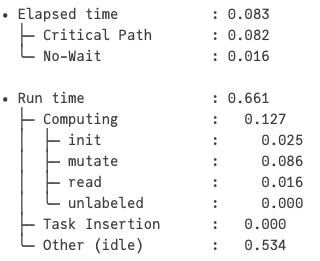
\includegraphics[width=0.3\textwidth]{figures/unicode-output.png}
  
% \end{frame}

% \begin{frame}[fragile]
% \frametitle{Logging}

% \begin{minted}[fontsize=\footnotesize]{julia}
% function work(A, B)
%   @dspawn init!(@W(A))               label="init A"
%   @dspawn init!(@W(B))               label="init B"
%   @dspawn mutate!(@RW(A))            label="mutate A"
%   @dspawn mutate!(@RW(B))            label="mutate B"
%   res = @dspawn result(@R(A), @R(B)) label="read A,B"
%   fetch(res)
% end
% using GraphViz
% GraphViz.Graph(log_info)
  
% \end{minted}
  
% \center 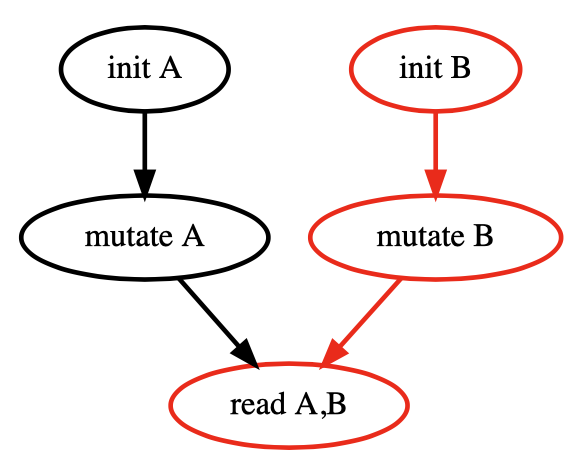
\includegraphics[width=0.3\textwidth]{figures/dag-output.png}
    
% \end{frame}

% \begin{frame}[fragile]
% \frametitle{Logging}

% \begin{minted}[fontsize=\footnotesize]{julia}
% function work(A, B)
%   @dspawn init!(@W(A))               label="init A"
%   @dspawn init!(@W(B))               label="init B"
%   @dspawn mutate!(@RW(A))            label="mutate A"
%   @dspawn mutate!(@RW(B))            label="mutate B"
%   res = @dspawn result(@R(A), @R(B)) label="read A,B"
%   fetch(res)
% end
% using CairoMakie # or GLMakie to benefit from more interactivity
% plot(log_info; categories=["init", "mutate", "read"])
    
%   \end{minted}
    
%   \center 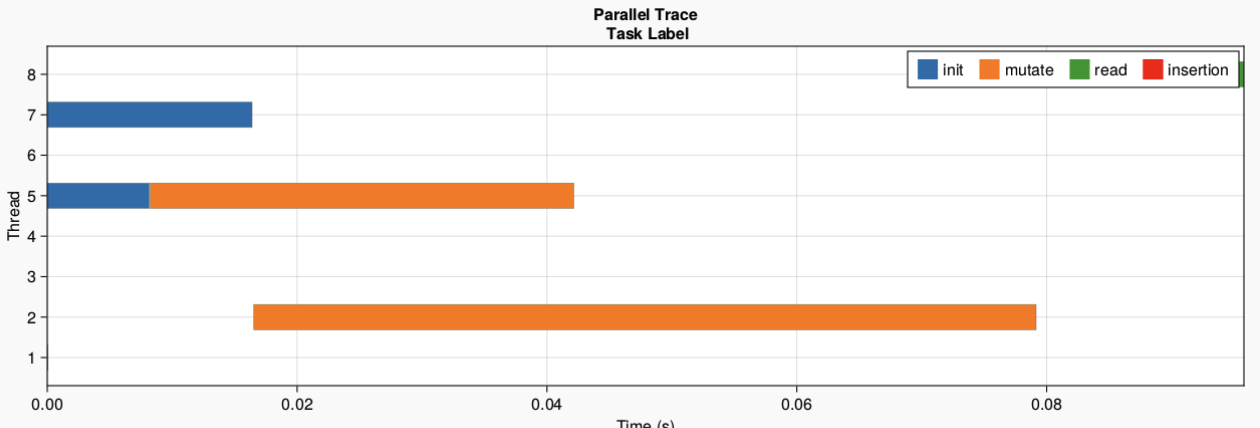
\includegraphics[width=0.8\textwidth]{figures/trace-output.png}
      
%   \end{frame}

\section{Real use case: tiled Cholesky}

\begin{frame}{Live examples}
  \begin{itemize} 
    \item \href{https://maltezfaria.github.io/DataFlowTasks.jl/dev/examples/cholesky/cholesky/}{Tiled cholesky factorization}
    \item
    \href{https://maltezfaria.github.io/DataFlowTasks.jl/dev/examples/blur-roberts/blur-roberts/}{Blur-Roberts filter}
    \item
    \href{https://maltezfaria.github.io/DataFlowTasks.jl/dev/examples/lcs/lcs/}{Longest
    common subsequence}
    \item
    \href{https://maltezfaria.github.io/DataFlowTasks.jl/dev/examples/sort/sort/}{Merge sort}
  \end{itemize}
\end{frame}

\section{Roadmap}

% \begin{frame}
% \frametitle{Summary}  

% \begin{itemize}
%   \item When \DFT{} is loaded a default \mintinline{julia}{TaskGraph}, with an
%   internal \mintinline{julia}{DAG}, is instantiated.
%   \item Upon creation, each \mintinline{julia}{DataFlowTask} object inserts
%   itself in the task graph.
%   \item Upon completion, each \mintinline{julia}{DataFlowTask} object inserts
%   itself in a finished channel
%   \item An asynchronous task is responsible for removing finished jobs from the graph
%   \item The \mintinline{julia}{@dspawn} macro provides a very convenient way to
%   create \mintinline{julia}{DataFlowTask}s
%   \item Logging is enabled using the \mintinline{julia}{@log} macro
% \end{itemize} 
% \end{frame}

\begin{frame}
\frametitle{Roadmap}  

\begin{itemize}
  \item Priority scheduling
  \item Nesting \mintinline{julia}{DataFlowTask}s
  \item ...
\end{itemize} 
\end{frame}


\end{document}